\setlength{\footskip}{8mm}

\chapter{Literature Review} 
\protect\label{ch:literature-review}

As said in the previous section, the goal of this study is to exploit \textit{deep learning} algorithms for face recognition in surveillance videos.

\section{About Deep Learning}
\protect\label{Main-keywords-of-the-topic}
According to \enquote{Deep Learning Methods and Applications} (Deng, Yu, 2014):

\blockquote{Deep learning is a set of algorithms in machine
learning that attempt to learn in multiple levels, corresponding
to different levels of abstraction. It typically uses artificial
neural networks. The levels in these learned statistical models
correspond to distinct levels of concepts, where higher-level concepts
are defined from lower-level ones, and the same lowerlevel
concepts can help to define many higher-level concepts.}

One of the most well-known deep learning algorithms is the \textit{Convolutional Neural Network} (LeCun, Bottou, Bengio and Haffner, 1998), a variant of the multilayer perceptron (Rosenblatt, 1961) which involves the use of convolutional layers (see Figure 2.1). Biologically inspired by mammalian visual mechanisms, convolutional neural networks are historically known for an application called \textit{LeNet}, able to recognize hand-written digits (LeCun et al., 1989). In the last 10 years, the interest in convolutional networks has grown quickly. In fact, with the evolution of technology --- basically massive usage of always more powerful GPU cards --- it has been possible to use these networks more widely and for various tasks. They have been used widely for human face classification tasks and have given impressive results.

\begin{figure}[!ht]
  \centering
  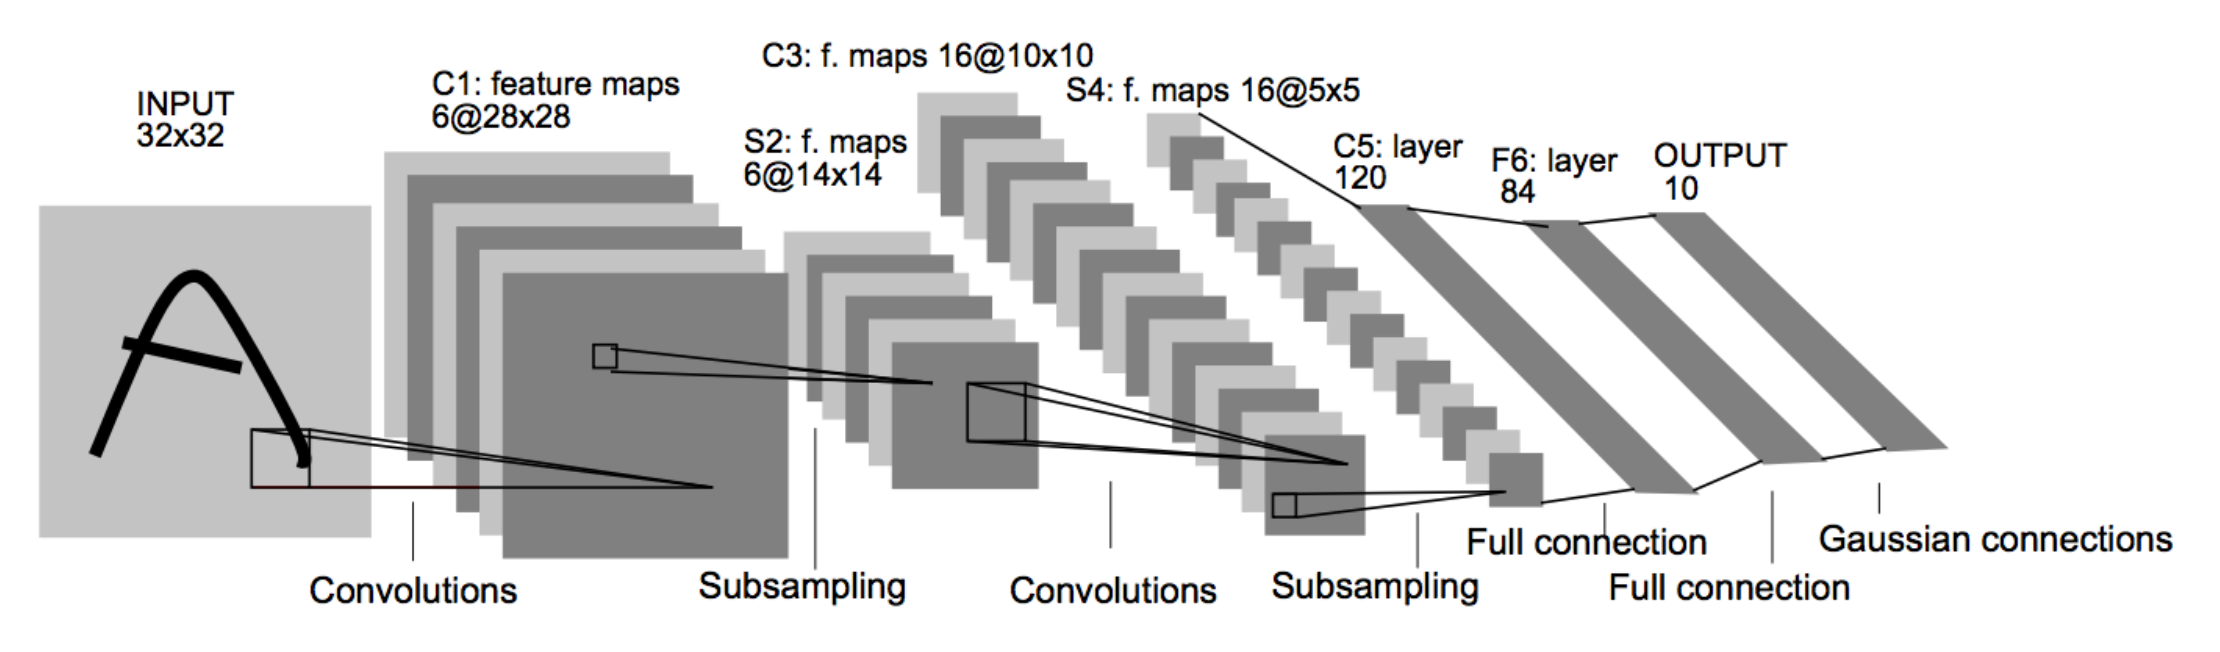
\includegraphics[scale=0.4]{figures/lenet.png}  
  \caption[Architecture of LeNet-5 for digit recognition. Extracted from LeCun, Bottou, Bengio and Haffner (1998).]{Architecture of LeNet-5 for digit recognition. Extracted from LeCun, Bottou, Bengio and Haffner (1998).}
  \protect\label{fig:lenet}
\end{figure}

\section{About Convolutional Neural Networks}

A convolutional neural network is generally made of one or more convolutional layers followed by a standard neural network.
Convolutional layers are similar to standard layers. The difference is that in this specific case, we connect only adjacent neurons of a layer to the next one, whereas, standard layers connect all the neurons of a layer to the next one. Then, most frequently a subsampling of the convolutional layer is applied and the output of this step is used as an input to the next layer.\\

The next figures show a typical convolutional neural network represented in 3 dimensions. Its role is to identify a hand-written digit in an image as an example of a particular written number. This 3D representation has been made by Harley, in 2015.\\

Figure 2.2 shows the full network. The bottom layer is the input, a hand-written \enquote{2} digit.


\begin{figure}[!ht]
  \centering
  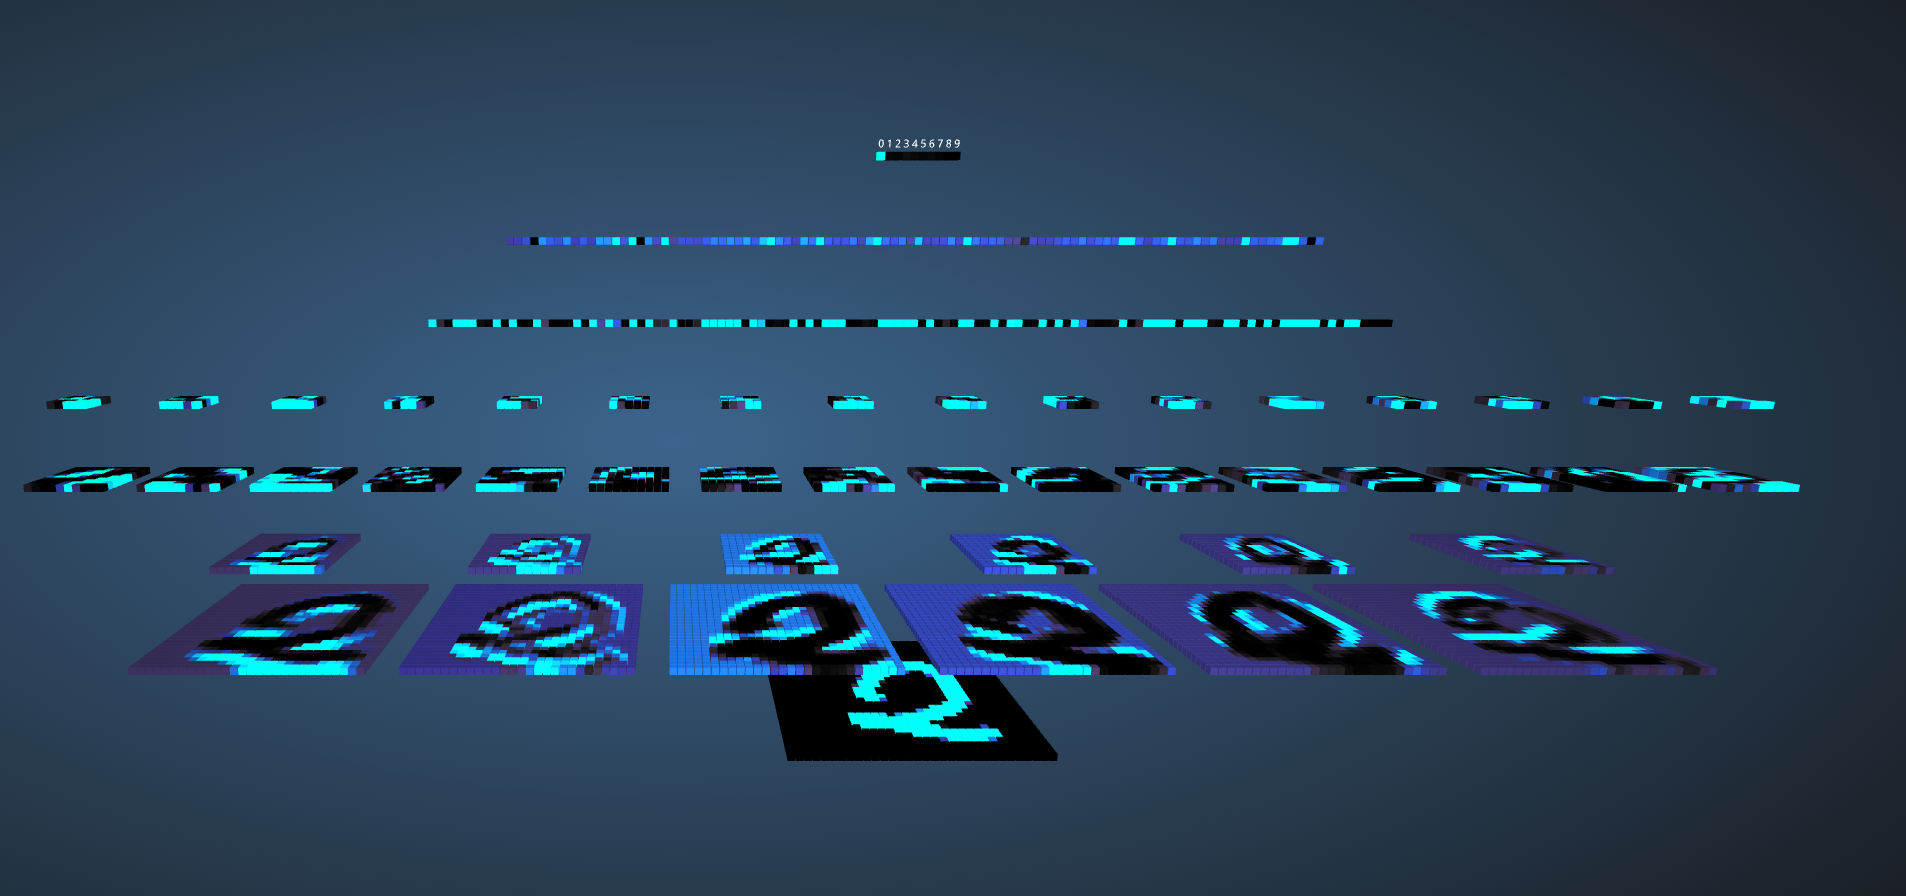
\includegraphics[scale=0.5]{figures/conv1.png}  
  \caption[3-dimensional representation of a typical convolutional neural network. Generated by Harley, 2015.]{3-dimensional representation of a typical convolutional neural network. Generated by Harley, 2015.}
  \protect\label{fig:conv1}
\end{figure}
\FloatBarrier

The next layer is the first convolutional one. See Figure 2.3. Some restricted sub-regions of the input are received by the neurons of the next layer. Convolutional units have tied weights, so that the same processing is applied at every local subregion of the input layer. This idea is biologically inspired by cells from the visual cortex of animals, which are sensitive to fixed small regions of the visual field and perform similar computation over the entire visual field.

\begin{figure}[!ht]
  \centering
  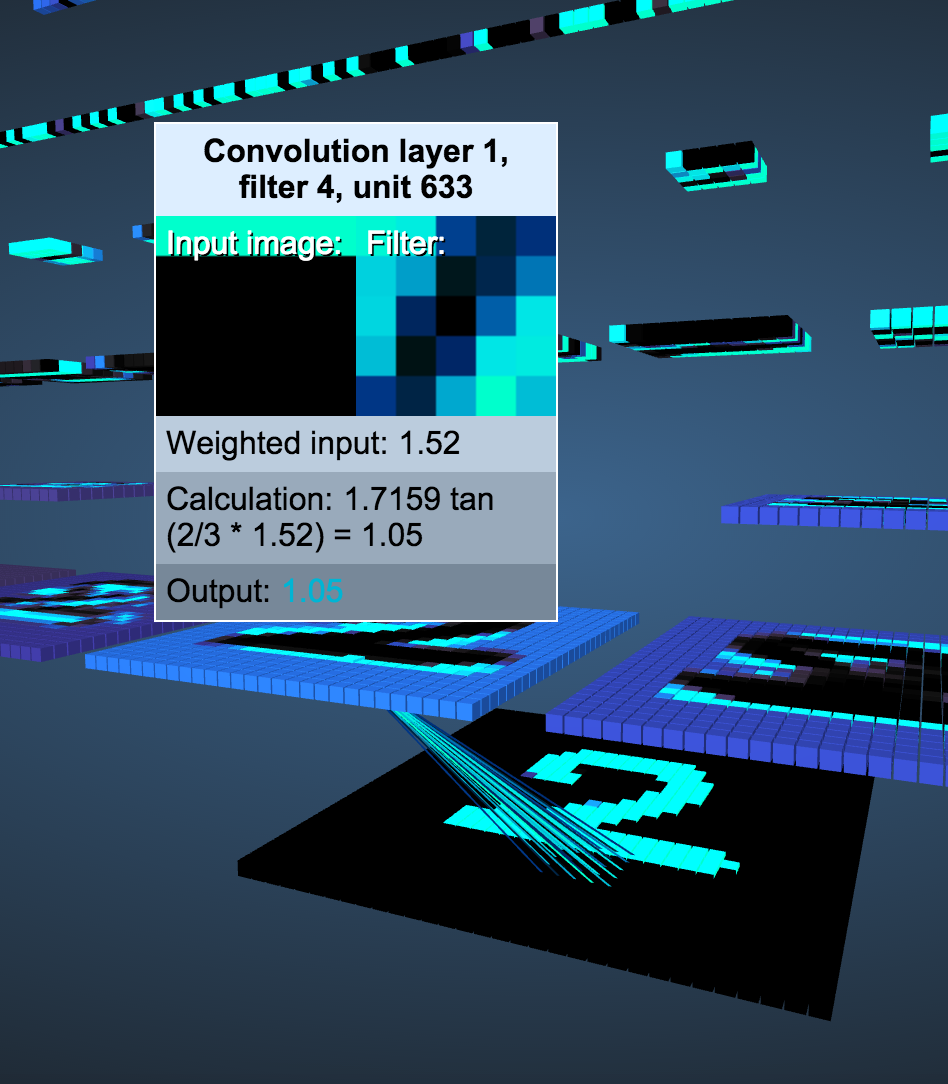
\includegraphics[scale=0.6]{figures/conv2.png}  
  \caption[The first convolutional layer. Generated by Harley, 2015.]{The first convolutional layer. Generated by Harley, 2015.}
  \protect\label{fig:conv2}
\end{figure}
\FloatBarrier
In the next layer of the convolutional network, subsampling occurs. Subsampling reduces sensitivity to small translations of similar features. Different types of subsampling exist. The most used is \enquote{max-sempling} which extracts the maximum value among the pixels of a region. See Figure 2.4. 

\begin{figure}[!ht]
  \centering
  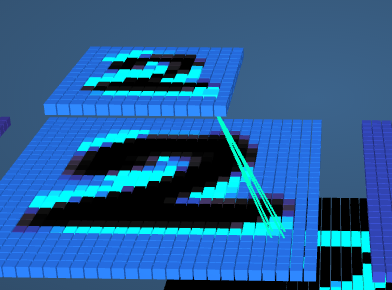
\includegraphics[scale=1.0]{figures/conv3.png}  
  \caption[The first subsampling layer. Generated by Harley, 2015.]{The first subsampling layer. Generated by Harley, 2015.}
  \protect\label{fig:conv3}
\end{figure}
\FloatBarrier
Figure 2.5 represents the second convolutional layer. Its input is the output of the first subsampling layer which represents the result of the computations of the first convolutional layer.

\begin{figure}[!ht]
  \centering
  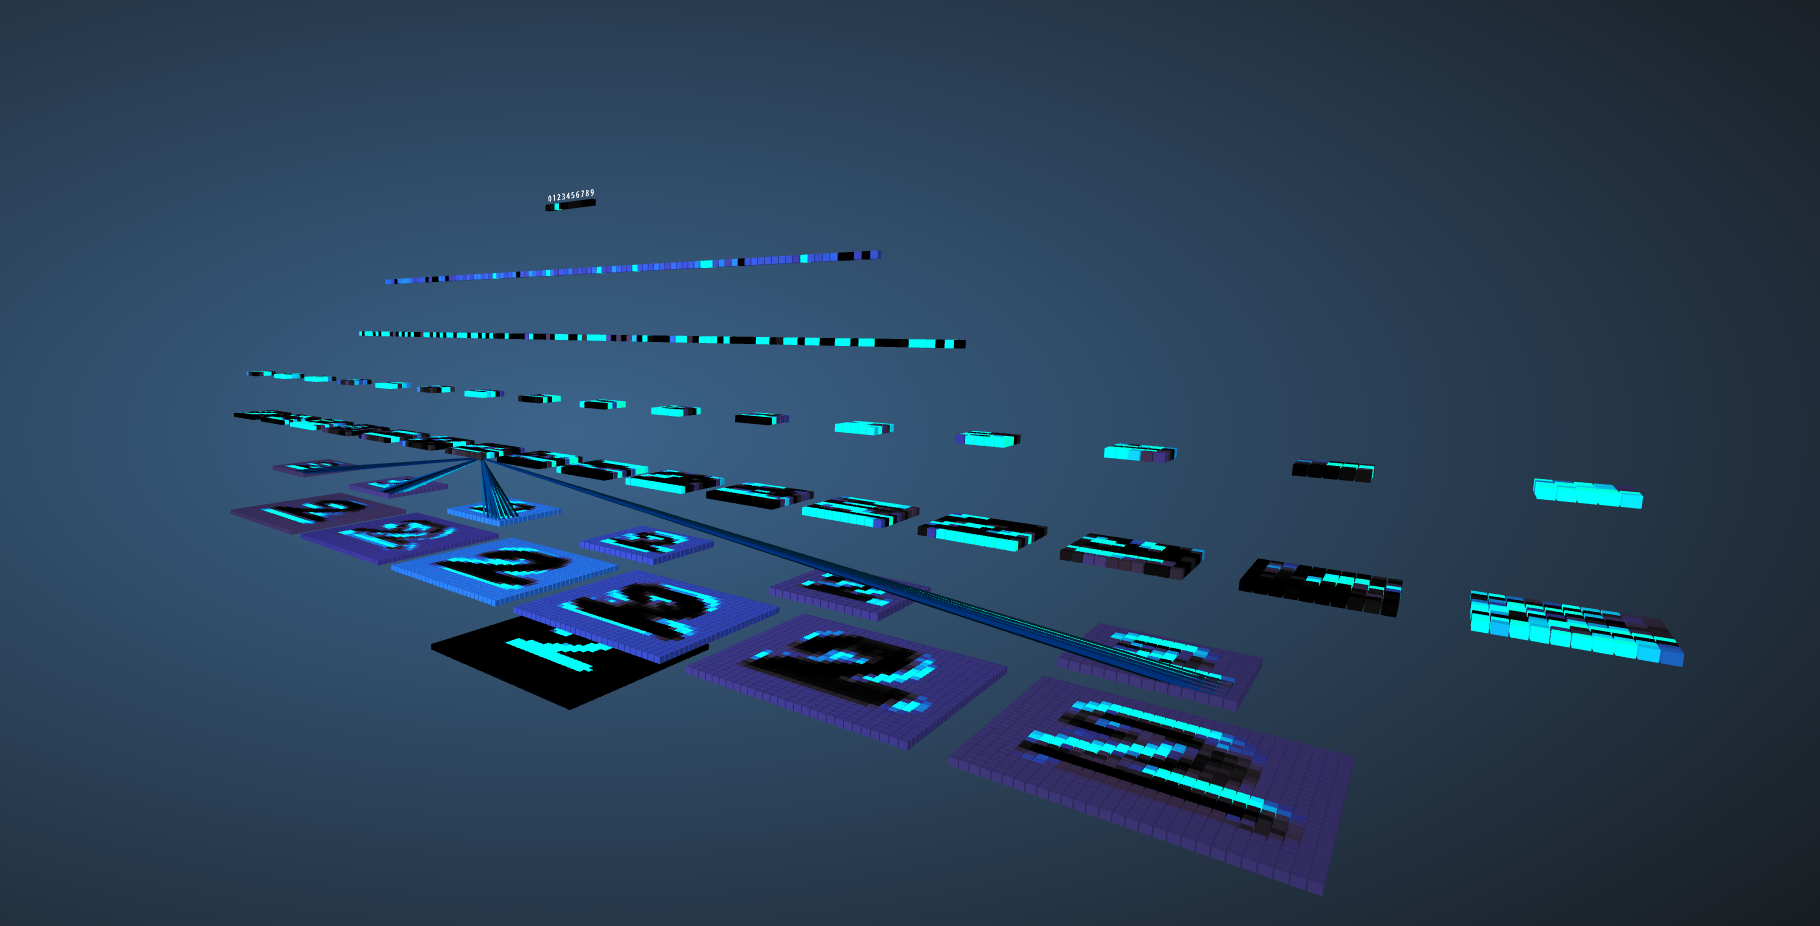
\includegraphics[scale=0.4]{figures/conv4.png}  
  \caption[The second convolutional layer. Generated by Harley, 2015.]{The second convolutional layer. Generated by Harley, 2015.}
  \protect\label{fig:conv4}
\end{figure}
\FloatBarrier
The two last layers before the final output represent standard fully-connected layers. See Figure 2.6.

\begin{figure}[!ht]
  \centering
  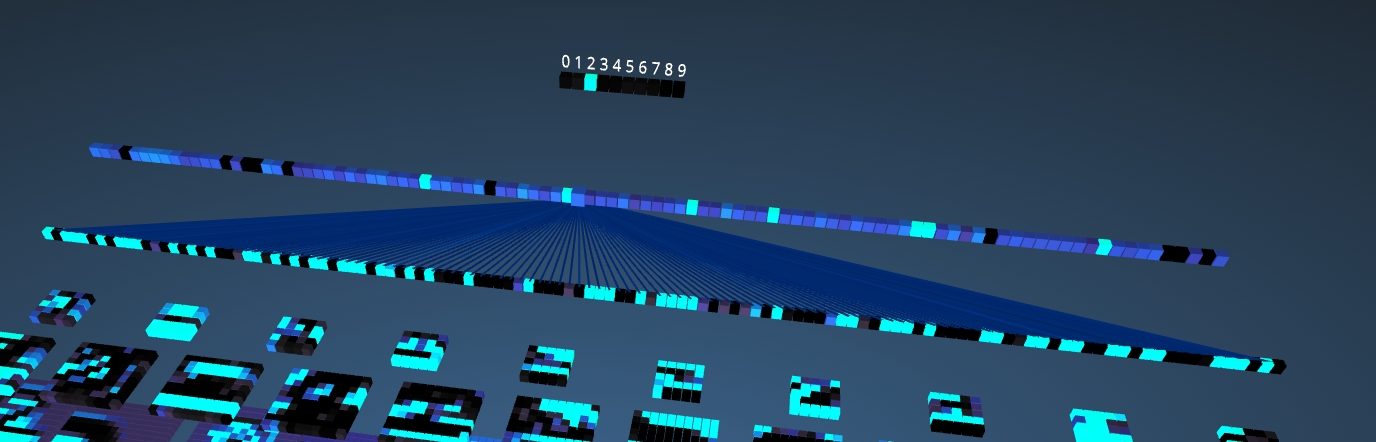
\includegraphics[scale=0.7]{figures/conv5.png}  
  \caption[The fully-connected layers. Generated by Harley, 2015.]{The fully-connected layers. Generated by Harley, 2015.}
  \protect\label{fig:conv5}
\end{figure}
\FloatBarrier

\section{Previous Work}
\subsection{Deep learning for face recognition}
There are two main schemes for face recognition:
\begin{itemize}
\item Recognition by person identification. In this case, a network takes an image as an input and returns a label that identifies one and only one person as an output. The literature on this type of architecture is extremely abundant. For face verification, DeepFace (Taigman, Yang, Ranzato, Wolf, 2014) reached 97.35\% accuracy on the Labeled Faces in the Wild (LFW) dataset. The state of the art for face identification is FaceNet (Schroff, Kalenichenko, Philbin, 2015).

\item Recognition by comparison. The \enquote{Same/Not Same} algorithms. The basic idea is that the training dataset is made of pairs of images linked to the label \enquote{1} if they represent the same object --- in our case, the face of a person --- and \enquote{0} otherwise. In deep learning, the standard same/not same network is called a \enquote{Siamese Network} (Chopra, Hadsell, LeCun, 2005). A Siamese network is built out of two convolutional networks. The input to the first is the first image of the pair and the input to the second is the second image. The two networks share the same parameters and return two values each. Those values are used to compute an energy. If the energy is high, the two images are considered to be \enquote{very different}. Otherwise they are considered to be \enquote{similar.} The energy is a function of a loss function used to update the parameters of the two convolutional networks by contrastive gradient descent (Figure \ref{fig:Siamese}). Intuitively, the computed energy is similar to gravitational potential energy. If a mass is far from Earth, its GPE is high, and the mass will be considered as not belonging to the planet. If the mass is stuck to the Earth, its GPE will be low, and the mass is considered part of the planet itself.


\begin{figure}[!ht]
  \centering
  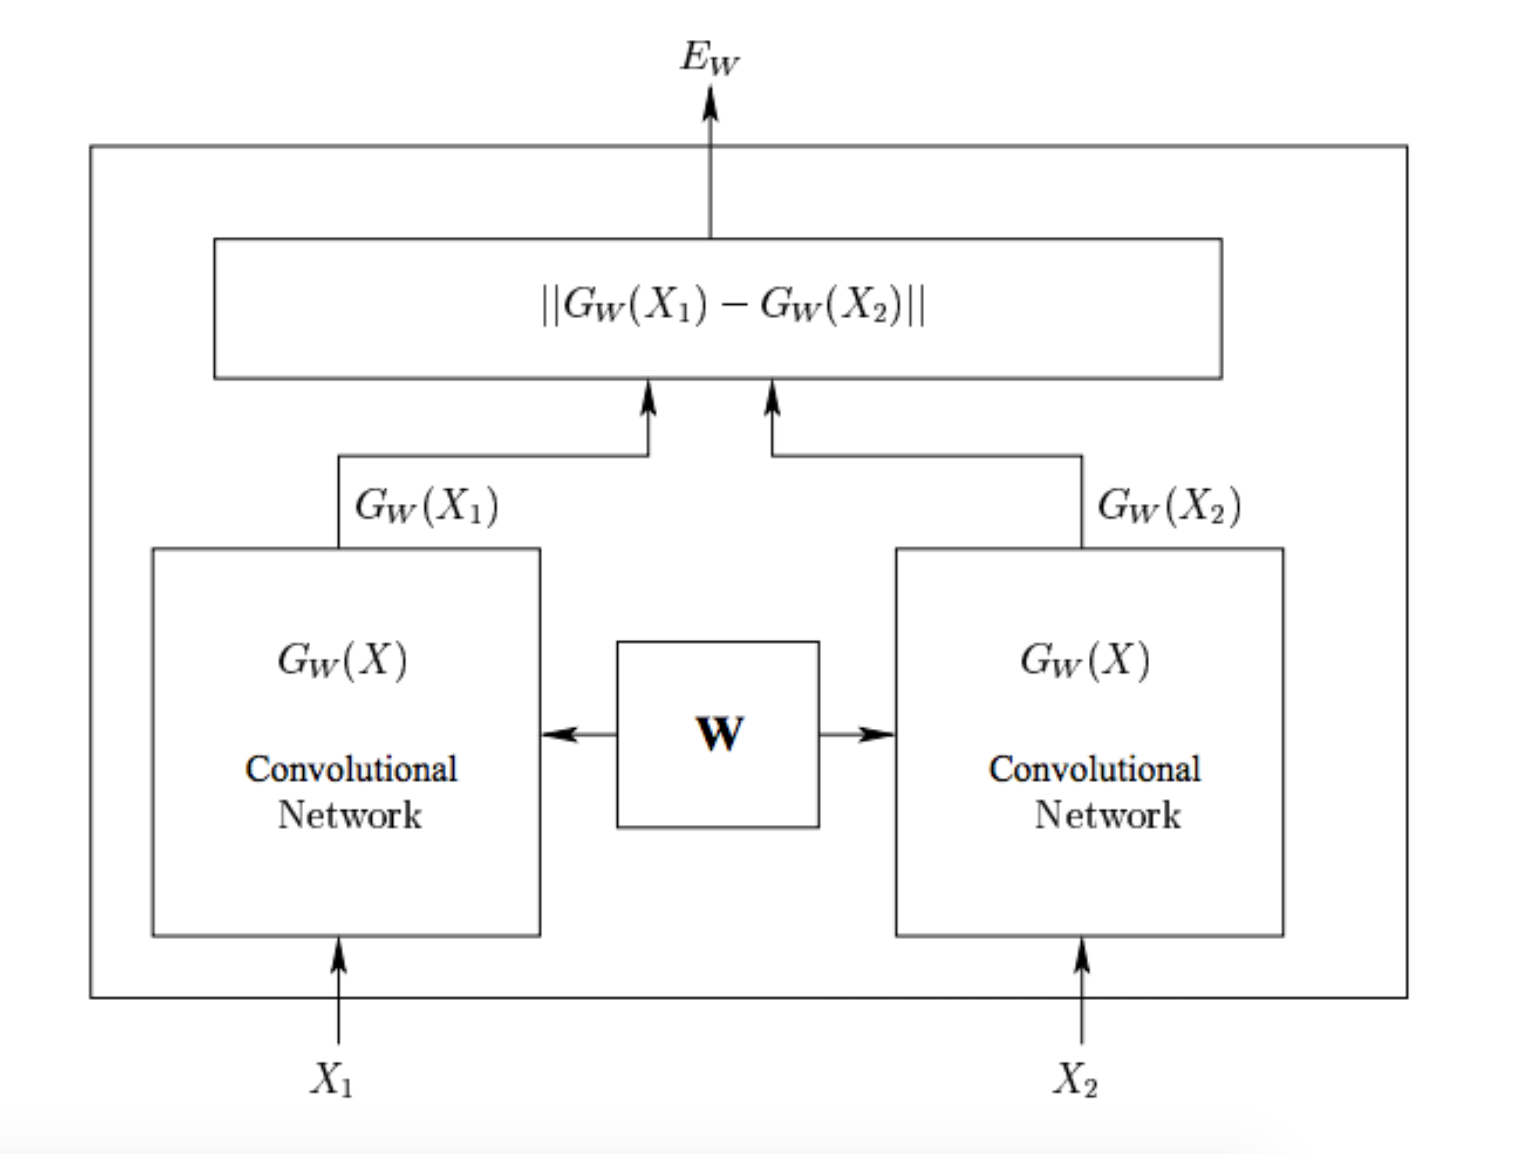
\includegraphics[scale=0.4]{figures/siamese.png}  
  \caption[Architecture of a Siamese network. Extracted from Chopra, Hadsell, LeCun, 2005.]{Architecture of a Siamese network. Extracted from Chopra, Hadsell, LeCun, 2005.}
  \protect\label{fig:Siamese}
\end{figure}
\FloatBarrier
\end{itemize}


\subsection{Video-Based Face Recognition}

On automated face recognition for surveillance video, a number of articles have been published. They are using a wide range of methods. Liu and Chen (2003) used a Hidden Markov Model for video-based face recognition. Le An, Kafai and Bhanu (2012) used a Dynamic Bayesian Network. Goswami, Bhardwaj, Singh and Vatsa (2014) proposed an interesting methodology. First, an algorithm extracts the most \enquote{memorable} frames in the video. Then, the chosen frame is applied to a deep learning network performing face recognition. This idea provides the state-of-the-art in low false acceptance rates.

\section{Conclusion}

Video-based face recognition is a very important area of research. Though many articles are published on this subject, some of the latest deep neural network techniques have yet to be applied to the context of images extracted from surveillance videos.